% LaTeX Template for Project Report, Version 2.0
% (Abstracted from a Major Project Report at CSED, NIT Calicut but can be
% modified easily to use for other reports also.)
%
% Released under Creative Commons Attribution license (CC-BY)
% Info: http://creativecommons.org/licenses/by/3.0/
%
% Created by: Kartik Singhal
% BTech CSE Batch of 2009-13
% NIT Calicut
% Contact Info: kartiksinghal@gmail.com
%
% It is advisable to learn the basics of LaTeX before using this template.
% A good resource to start with is http://en.wikibooks.org/wiki/LaTeX/
%
% All template fields are marked with a pair of angular brackets e.g. <title here>
% except for the ones defining citation names in ref.tex.
%
% Empty space after chapter/section/subsection titles can be used to insert text.
%
% Just compile this file using pdflatex after making all required changes.

\documentclass[12pt,a4paper,margin=0in]{report}
\usepackage[pdftex]{graphicx} %for embedding images
\usepackage{url} %for proper url entries
\usepackage[bookmarks, colorlinks=false, pdfborder={0 0 0}, pdftitle={A
Fencing Competition Results Service}, pdfauthor={Matthew Carus},
pdfsubject={BSc Computing and IT}, pdfkeywords={Open University,
Computing, IT, Report, TM470}]{hyperref}
%for creating links in the pdf version and other additional pdf attributes, no effect on the printed document \usepackage[final]{pdfpages} %for embedding another pdf, remove if not required
\usepackage{listings} %for including source code
\usepackage{color} %for including source code

\usepackage[round]{natbib}
\bibliographystyle{abbrvnat}
\setcitestyle{authoryear,open={(},close={)}}

\begin{document}
\renewcommand\bibname{References} %Renames "Bibliography" to "References" on ref page

%include other pages
\begin{titlepage}

\begin{center}

\textup{\small {\bf TM470 Project Report}}\\[0.2in]

% Title
\Large \textbf {A Fencing Competition Results \\ Web Service}\\[0.2in]

       \small \emph{Submitted in partial fulfillment of\\
        the requirements for the award of the degree of}
        \vspace{.2in}

       {\bf Bachelor of Science \\in\\ Computing and IT}\\[0.2in]

% Submitted by
\normalsize Submitted by \\
\begin{table}[h]
\centering
\begin{tabular}{lr}\hline 
\\
Matthew Anthony Carus & B3951972 \\ \\ \hline 
\end{tabular}
\end{table}

\vspace{.1in}
Under the guidance of\\
{\textbf{Prof. Peter Smith}}\\[0.2in]

\vfill


% Bottom of the page
% 
\includegraphics[width=0.36\textwidth]{Open_University_coat_of_arms}\\[0.1in]

%\begin{minipage}[t][][t]{0.45\textwidth}
\begin{center}
%
\includegraphics[width=3cm]{ou_cmyk_masterlogo_29mm.jpg}\\[0.4in]

\includegraphics[width=3cm]{Open_University_coat_of_arms.png}\\[0.4in]
\Large{Department of Computing and IT}\\
\normalsize
\textsc{The Open University}\\
Milton Keynes, United Kingdom \\
\vspace{0.2cm}
\end{center}
%\end{minipage}%
%\begin{minipage}[t][][t]{0.45\textwidth}
\begin{center}
\textsc{In collaboration with}\\[0.2in]

\includegraphics[width=3cm]{british-fencing.png}\\[0.1in]
\Large{British Fencing}\\
\normalsize
London, United Kingdom \\
\vspace{0.2cm}
\end{center}
%\end{minipage}%

\end{center}


\end{titlepage}

\newpage
\thispagestyle{empty}

\begin{center}

\huge{Department of Computing and IT}\\[0.5cm]
\normalsize
\textsc{The Open University}\\[2.0cm]

\emph{\LARGE Certificate}\\[2.5cm]
\end{center}
\normalsize This is to certify that this is a bonafide record of the project
presented by the student whose name is given below during 2016 in partial fulfilment of the requirements of the degree of Bachelor of Science in Computing
and IT.
[1.0cm]
\begin{table}[h]
\centering
\begin{tabular}{lr}
Student Name & PI Number \\ \\ \hline

Matthew Anthony Carus & B3951972
\end{tabular}
\end{table}

\vfill


% Bottom of the page
\begin{flushright}
<Tutor name here>\\
(Tutor)\\[1.5cm]
Leonor Barroca \\
(Module Team Chair)
[1.5cm]
\today
\end{flushright}
\vspace{2in}
\begin{abstract}

<Abstract here>

\end{abstract} 


\pagenumbering{roman} %numbering before main content starts
\tableofcontents
\listoffigures

\newpage
\pagenumbering{arabic} %reset numbering to normal for the main content

\chapter{Problem Definition}

<Problem Definition here>
 %objective changed to problem definition
\chapter{Introduction}

\section{Background and Recent Research}
\subsection{<any sub section here>}

\subsection{Literature Survey}

\subsubsection{<Sub-subsection title>}
some text \citep{knuthwebsite} \citet{latexcompanion}, some more text

\subsubsection{<Sub-subsection title>}
even more text\footnote{<footnote here>}, and even more.

\section{Motivation}
 %literature survey included in this
\chapter{Project Plan}

% \section{Gantt Chart}
% \def\svgwidth{350px}
%\input{gantt.pdf_tex}
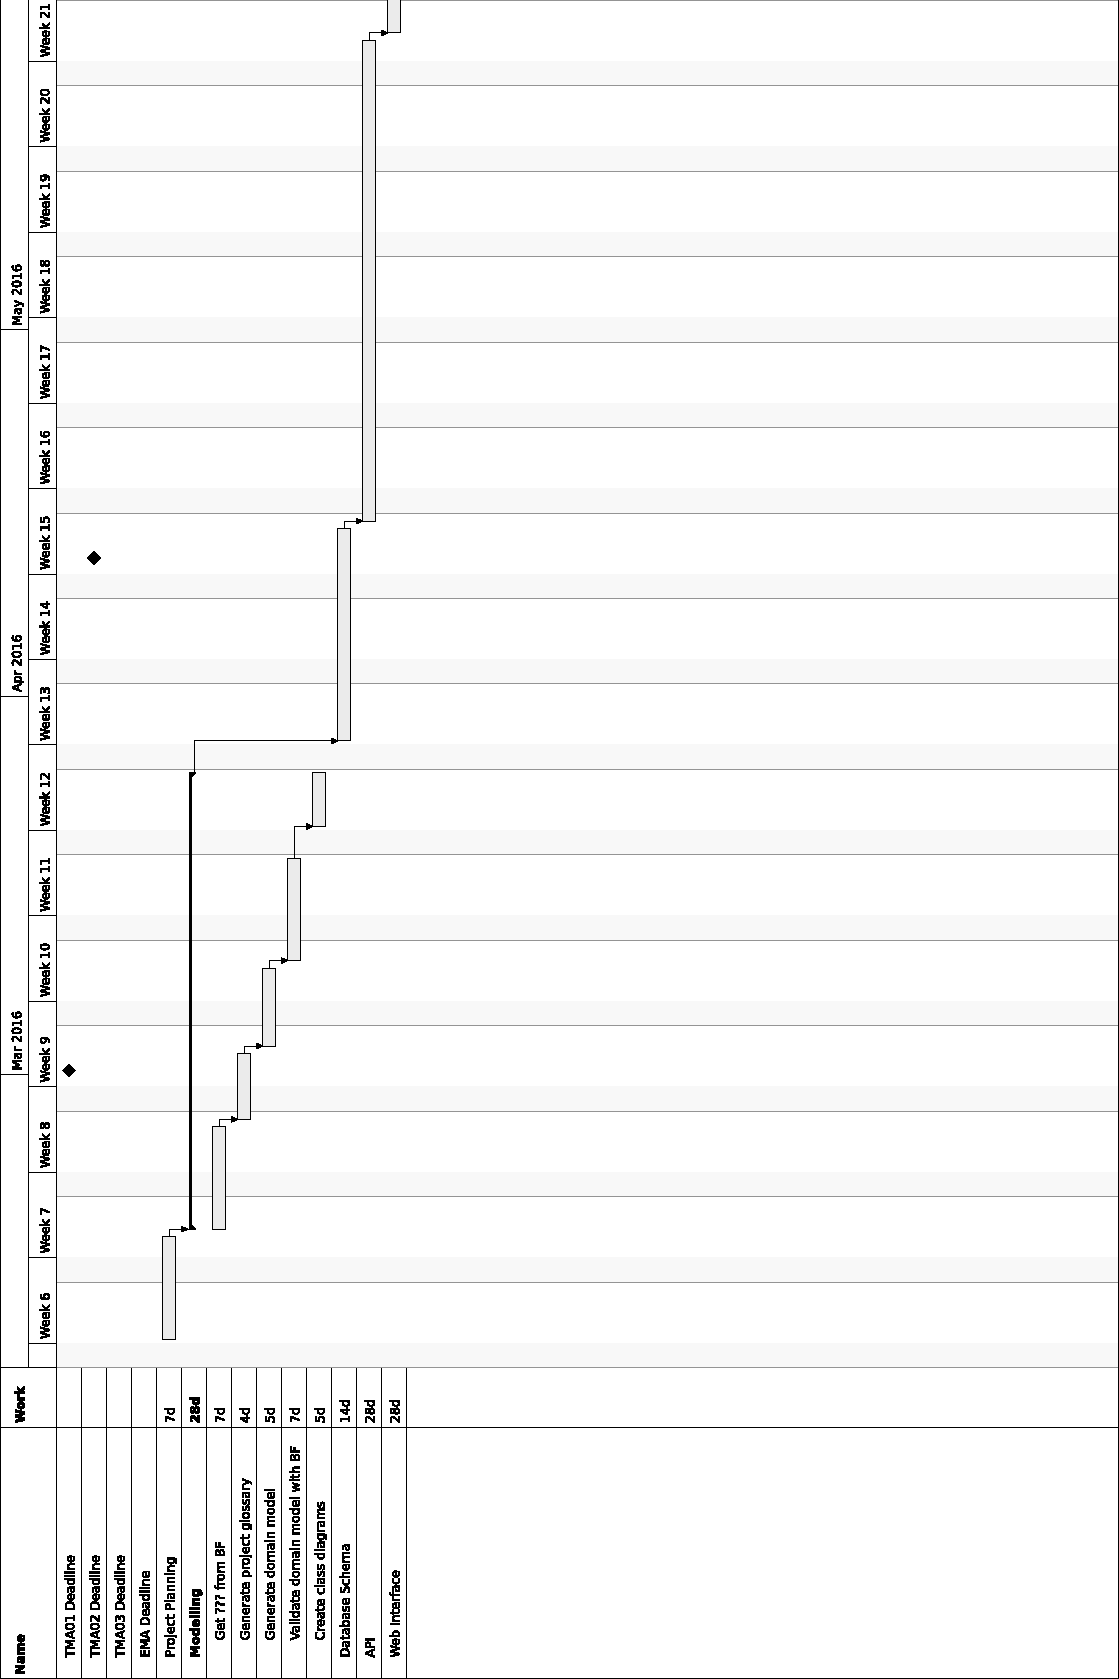
\includepdf{gantt-p1.pdf}
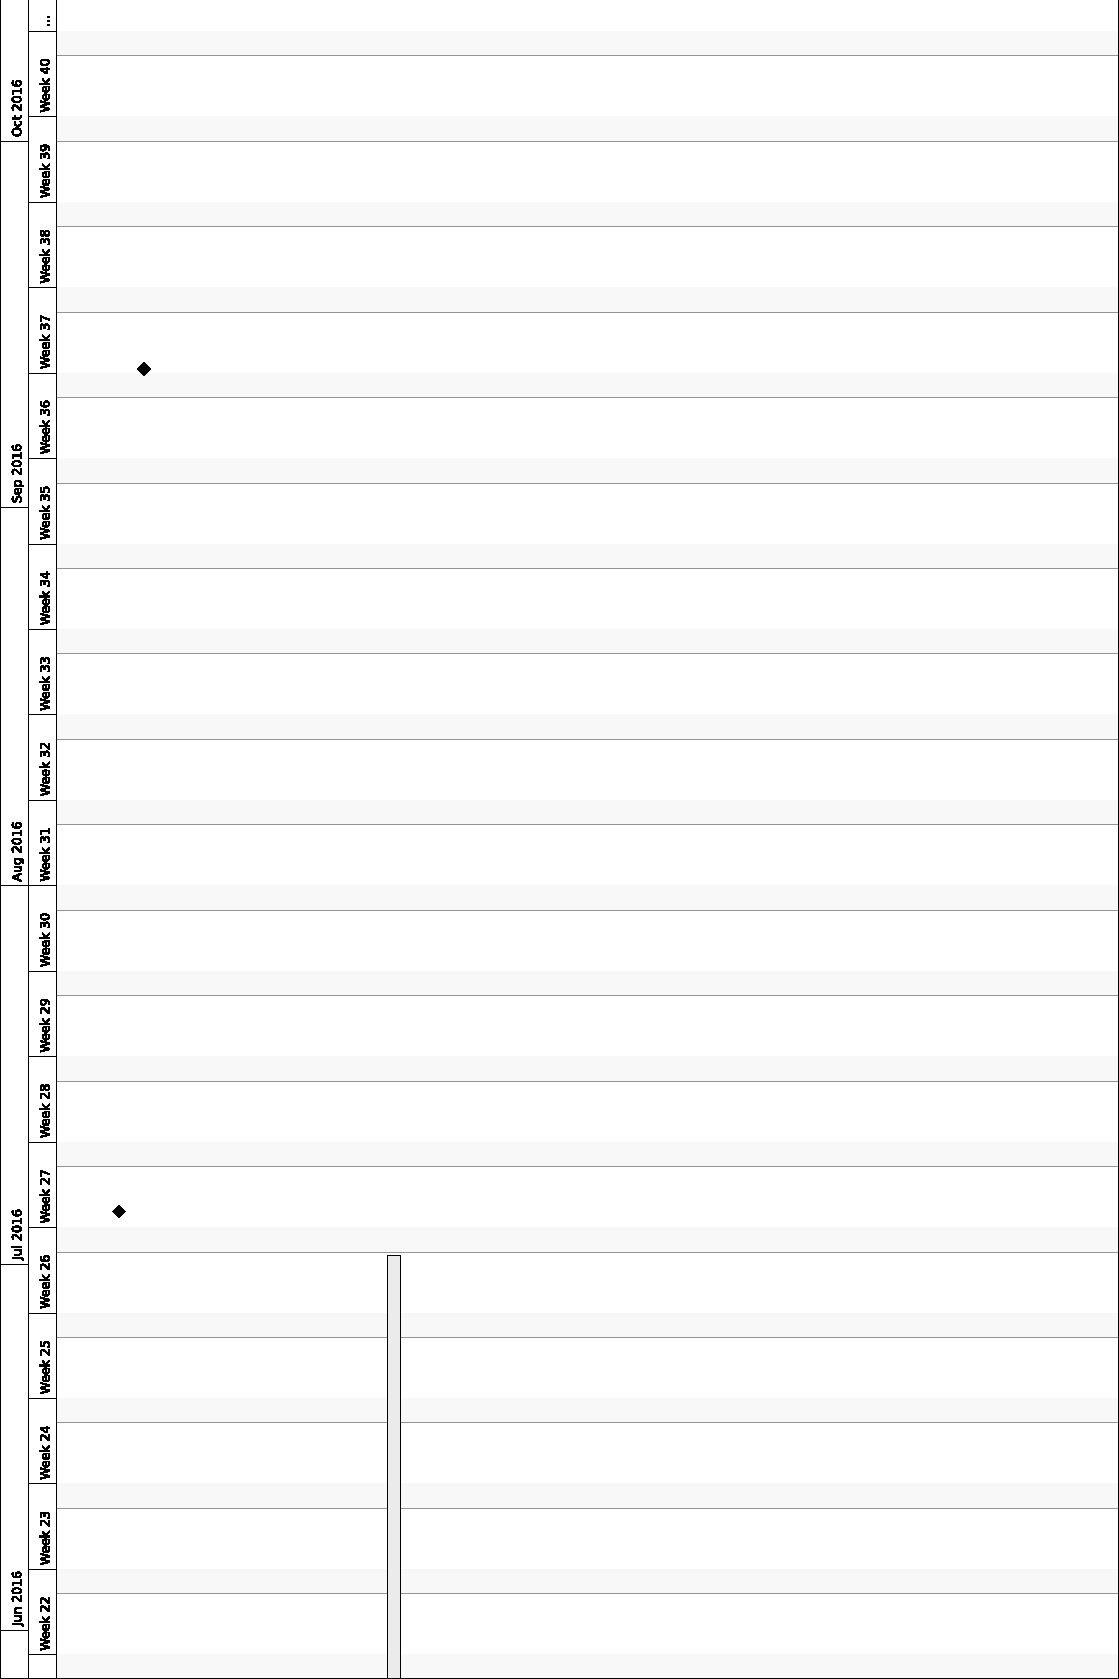
\includepdf{gantt-p2.pdf}
\chapter{Models}
\section{Grammatical Parse} \label{section:gramaticalParse}
After consultation with British Fencing, I was directed to a useful resource
which describes how fencing competitions operate \citep{bfcompguide}. Not
all of this document is relevant but the sections that are are reproduced
below, with \textbf{nouns} in bold and \underline{verbs} underlined. Only the
nouns and verbs deemed to be directly relevant to the process of competing in a
competition have been included.
\begin{displayquote}
Check In: All \textbf{competitions} start by \textbf{fencers}
visiting the \textbf{check in desk} \underline{to confirm} that they
are present. Don’t miss this bit out - your \textbf{entry}
will \underline{be scratched}.
When \underline{checking in}, \textbf{fencers} are required to show
their \textbf{British Fencing card}. See the box (right) for
details. This carries \textbf{insurance}. Without it, you
may not fence. Fencing usually starts about 30 - 60 minutes
after \underline{check in} closes.
Pools: After \textbf{check in}, \textbf{competitors} are divided
into “\textbf{pools}” - groups of 5 - 7 \textbf{fencers} who all
\underline{fence} each other up to 5 \textbf{hits}. (4 \textbf{hits} for some
under 9 \textbf{competitions}). Time is limited to 2 or 3
minutes. Sometimes there may be two rounds of
\textbf{pools}, particularly in \textbf{age group competitions}.
Direct Elimination: The \textbf{results} of the \textbf{pools}
are used to \underline{seed} the \textbf{knockout phase} of the
\textbf{competition}. In some \textbf{competitions}, up to 30\%
of the \textbf{fencers} who did worst are \underline{eliminated}, but
in most cases all \textbf{fencers} \underline{go through} to the \textbf{direct
elimination (DE)} stage.
The \textbf{DE} rewards \textbf{fencers} who do well in the
\textbf{pool} stages, and keeps the strong \textbf{fencers} apart
until near the end of the \textbf{competition}. In a
\textbf{competition} with 64 \textbf{entrants}, the first round of
DEs would see 1st place fence 64th, 2nd place
fence 63rd and so on. If the number of
\textbf{entrants} is not a power of 2, (ie 8, 16, 32, 64
etc) then those \textbf{fencers} who did best in the \textbf{pools}
will \underline{get a “\textbf{bye}”} through the first \textbf{DE} round. After
several \textbf{DE} rounds, there will only be two \textbf{fencers}
left - the \textbf{finalists}.
\textbf{Direct elimination} fights are up to 15 \textbf{hits} (adults)
10 \textbf{hits} (under 13s) or 8 \textbf{hits} (under 9s). \textbf{DE fights}
are normally 3 x 3 minutes (sometimes less for \textbf{younger
fencers}) with a 60 second break between \textbf{periods}.
\end{displayquote}
\section{Project Glossary} \label{section:projectGlossary}
From the grammatical parse in section \vref{section:gramaticalParse} a project
glossary can be compiled. As a part of this, I removed all duplicate words,
plurals and synonyms, choosing the most appropriate word from any sets of synonyms as the noun or verb to represent
that entity/action. Note that synonyms in this sense are not necessarily true
synonyms but are equivalent terms in the context of fencing and fencing
competitions. Objects that have been identified as being a synonym of another
object, but not a complete synonym have had \textit{(sub-type)} appended to them
in the synonym list. The description of the words comes either from the text
above, from basic internet searching, or from my own knowledge of the sport.
\begin{center}
\begin{longtable}[l]{| p{.20\textwidth} | p{.80\textwidth} |} 
 \caption{\label{tab:ProjectGlossary}Project Glossary}
\hline
\textbf{Nouns} & \\ 
 Competition & An over-arching event at which one or more events
 take place \\
 & \textit{synonyms: age group competition (sub-type)} \\ 
 Fencer & An individual (human being) who competes in a fencing
 competition \\
 & \textit{synonyms: competitor, entrant, finalists (sub-type),
 younger fencers (sub-type)} \\
 Check-in desk & The location that fencers present themselves to
 in order to confirm that they will take part in a competition \\
 Entry & The link between a fencer and a competition \\
 British Fencing Card & A form of identity card indicating that a
 fencer has membership of British Fencing, and by extension is insured to
 compete \\
 & \textit{synonyms: insurance} \\
 Hit & The act of one fencer striking another and scoring a point \\
 Result & A listing of fencers in order of their measured performance in a 
 particular round \\
 Direct Elimination & The phase of a competition where defeating
 another fencer results in their elimination from the competition and your
 promotion to the next round. \\
 & \textit{synonyms: DE, knockout phase} \\
 Bye & The act of progressing through a round of the Direct
 Elimination stage of the competition without having to face another fencer.
 This is used in the event that the number of fencers is not a power of 2. \\
 Bout & An individual fencing match between two fencers \\
 & \textit{synonyms: fight} \\
 Period & A time-based subdivision of a bout \\
 Poule & A small grouping of fencers who all fence against one
 another in a series of bouts. \\
 & \textit{synonyms: pool} \\ 
 Event & A tournament in which fencers of the same gender, age
 group and weapon fence \\
 \textbf{Verbs} & \\
 Check In & The act of a fencer confirming that they have arrived at the venue
 of the competition and they intend to compete in it. \\
 & \textit{synonyms: to confirm (attendance at the competition)} \\
 Be Scratched & To be removed from the competition without competing \\
 Fence & The act of one fencer engaging in a fencing bout with another fencer \\
 & \textit{synonyms: fight} \\
 Seed & To use the results of one or more round(s) of competition to determine
 the structure of the next round. \\
 Eliminated & To be removed from the competition as a result of loosing a bout
 in a Direct Elimination round, or (in some cases) not being ranked high enough
 after a round of Poules \\
 Go Through & To progress from one round to the next, either by being ranked
 high enough after a poules round, or by winning a Direct Elimination bout \\
 Get a Bye & Be in receipt of free passage from one round of Direct
 Elimination to the next, without having to face another fencer. This is used in
 the case that the number of competitors in a round of Direct Elimination is not
 a power of 2 \\
 \hline
\end{longtable}
\end{center}
\section{Business Processes} \label{section:businessProcesses}
I have decided that for the purposes of this project, modelling the business
processes associated with the process of a fencer taking part in a competition
is not appropriate. The reason for this is that the software system will not
seek to implement these processes, but rather be an archive or the results of
these processes. Other software (such as Engarde and Fencing Time, mentioned in
section \vref{chapter:research}) already implement these processes. The
business processes that I will model will be the process by which data gets
added to the system and viewed by users of the system.
\section{Use Case Diagram} \label{section:useCaseDiagram}
\begin{figure}[!ht]
  \centering
  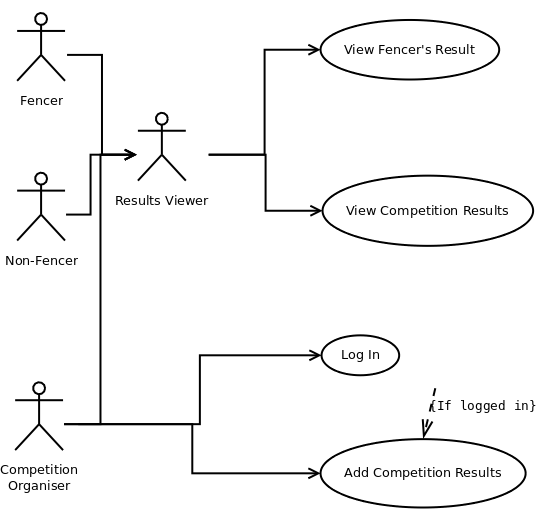
\includegraphics[width=10cm]{use_case_diagram.png}
  \caption{Use Case Diagram}
\end{figure}
\section{Class Diagram} \label{section:classDiagram}
As mentioned above, the project glossary includes terms relating to the actual
competition process. Some of these terms are relevant to a results hosting
service and some are not. Terms like \textit{Check-in desk} and
\textit{British Fencing Card } are only relavent during the actual competition
itself, therefore I have excluded them from the class diagram in
\vref{fig:classDiagram}.
\begin{figure}[!ht]
  \centering
  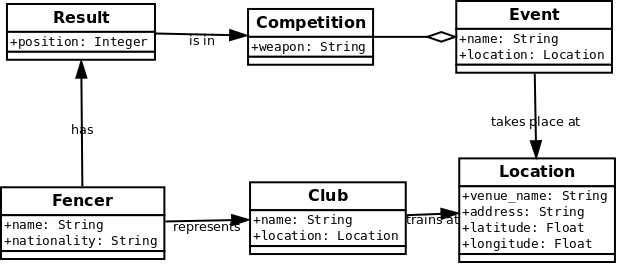
\includegraphics[width=10cm]{class_diagram.png}
  \caption{Class Diagram}
  \label{fig:classDiagram}
\end{figure}
\begin{figure}[!ht]
  \centering
  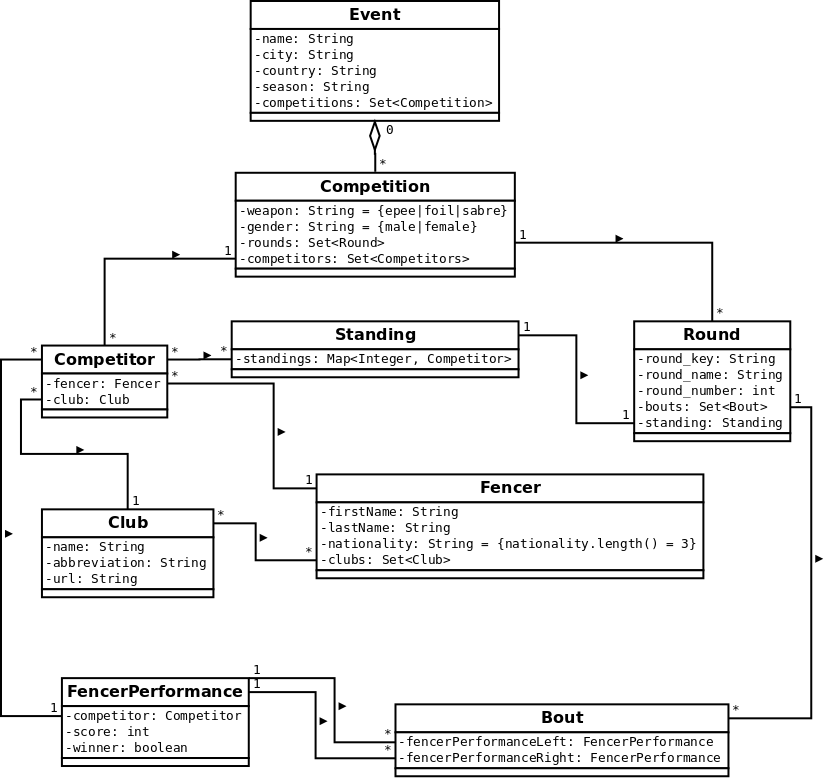
\includegraphics[width=12cm]{class_diagram_full.png}
  \caption{Full Class Diagram}
  \label{fig:classDiagramFull}
\end{figure}
\begin{figure}[!ht]
  \centering
  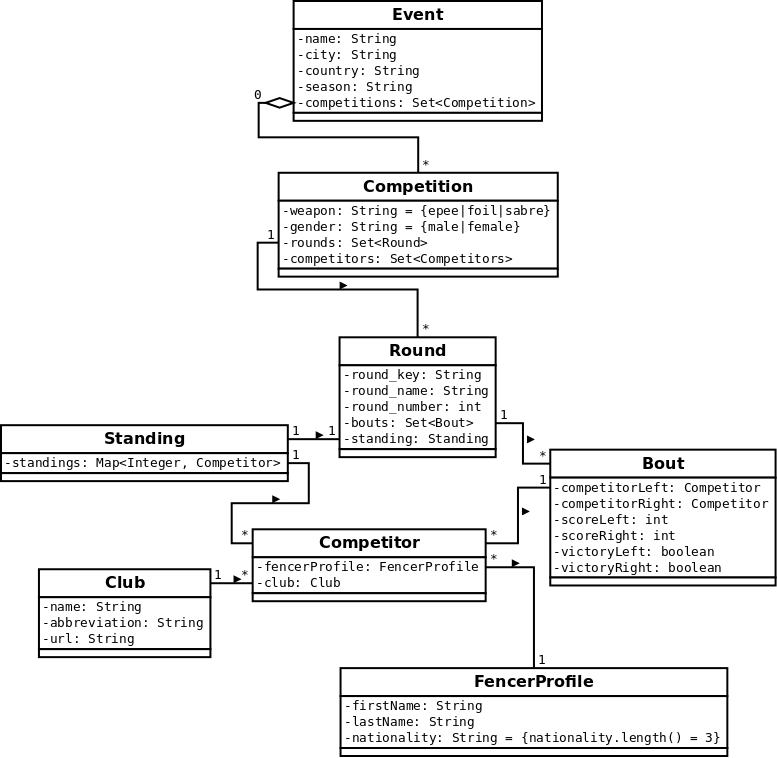
\includegraphics[width=10cm]{class_diagram_reduced.png}
  \caption{Reduced Class Diagram}
  \label{fig:classDiagramFull}
\end{figure}
The class diagrams in \vref{fig:classDiagramGeneratedNetFencingarchive}\footnote{Also available at
  http://github.com/mattcarus/something/here.png} and
\vref{fig:classDiagramGeneratedSportsml}\footnote{Also available at
  http://github.com/mattcarus/something/here.png} reflects what was actually coded in the
\(net.fencingarchive\) and \(sportsml\) packages and were generated
automatically (but re-arranged manually).
\begin{figure}[!ht]
  \centering
  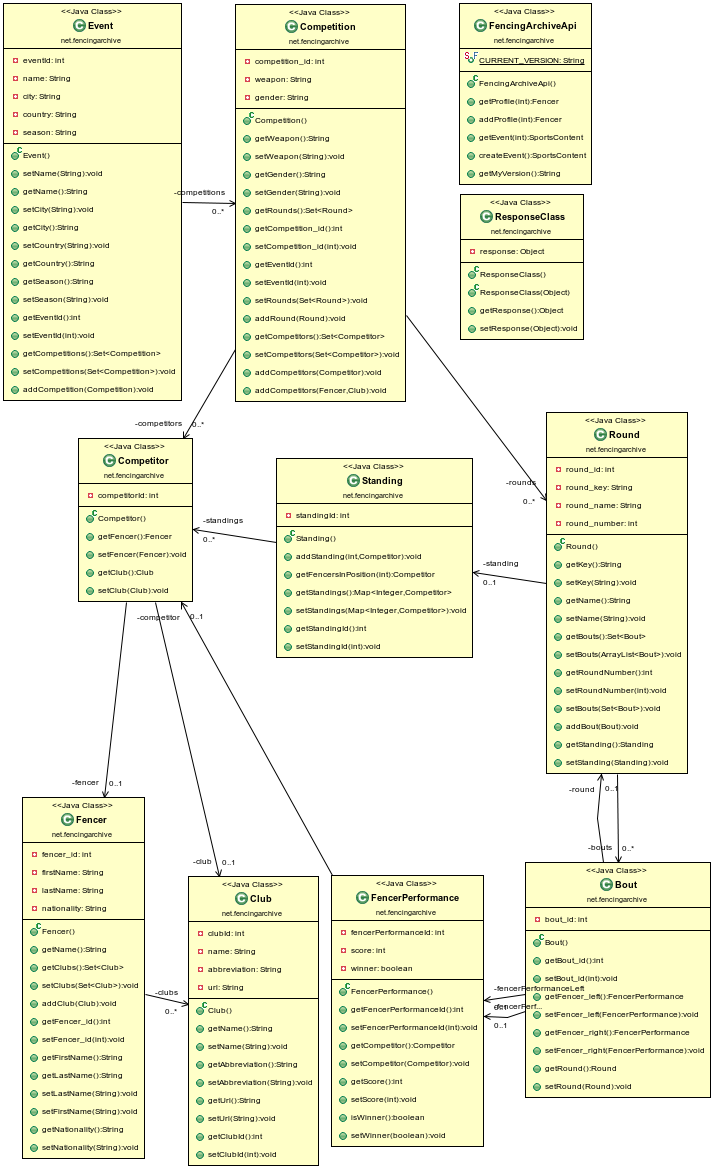
\includegraphics[width=\textwidth,height=0.9\textheight,keepaspectratio]{ObjectAid/class-diagram.png}
  \caption{net.fencingarchive Class Diagram - Generated from source code}
  \label{fig:classDiagramGeneratedNetFencingarchive}
\end{figure}
\begin{figure}[!ht]
  \centering
  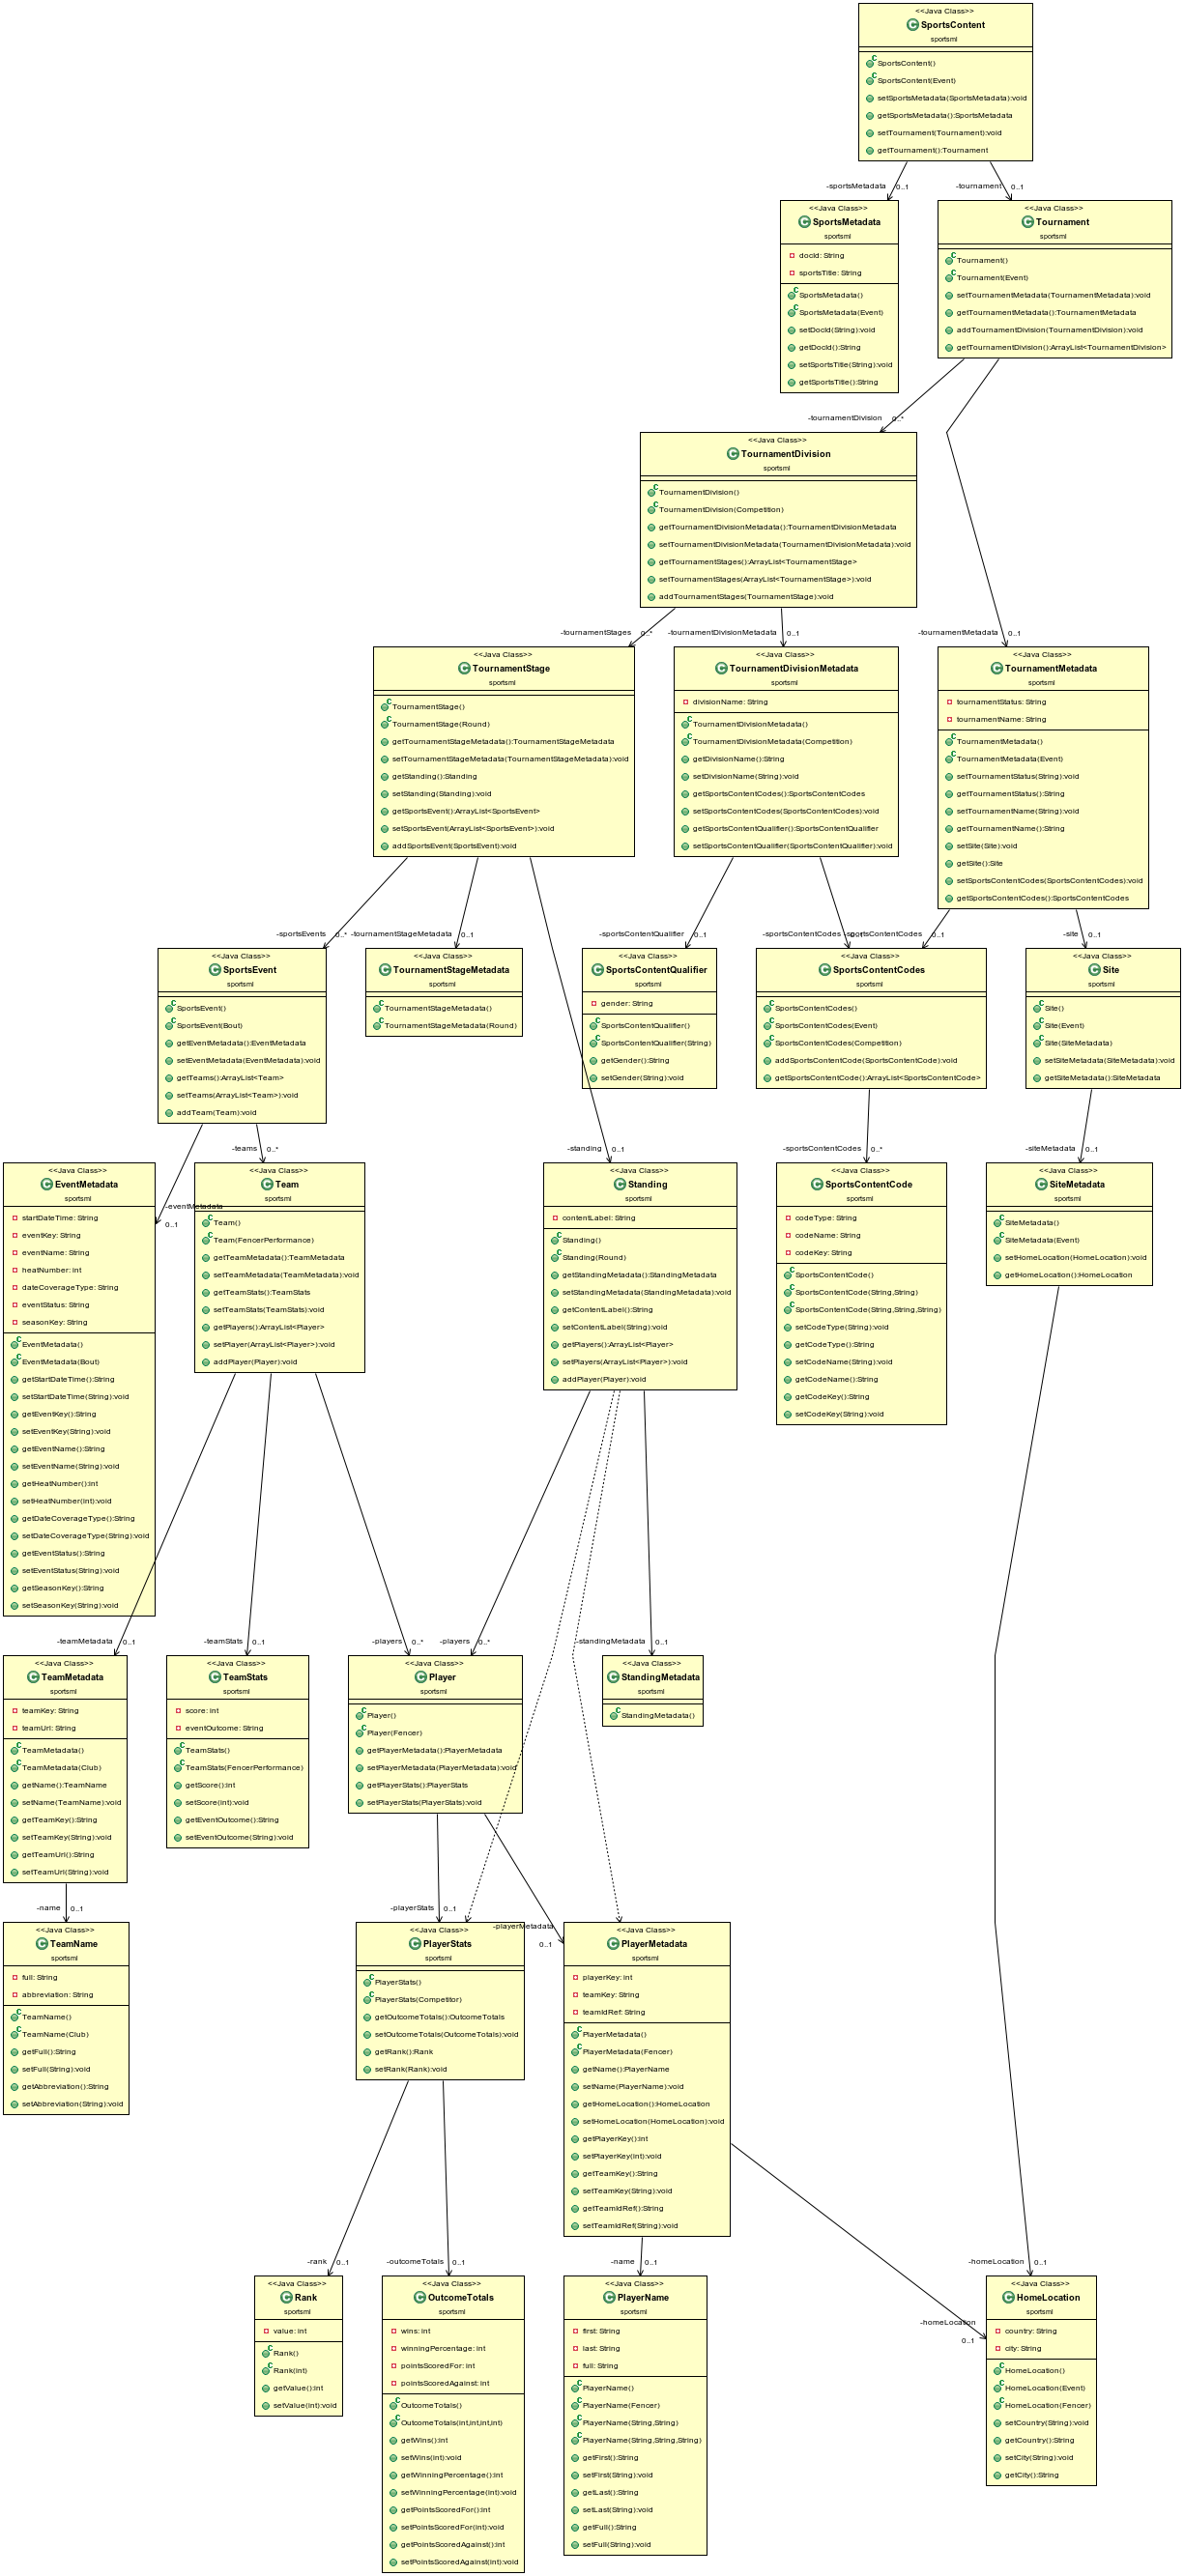
\includegraphics[width=\textwidth,height=0.9\textheight,keepaspectratio]{ObjectAid/class-diagram-sportsml.png}
  \caption{sportsml Class Diagram - Generated from source code}
  \label{fig:classDiagramGeneratedSportsml}
\end{figure}
\section{Database Design} \label{sectiondatabaseDesign}
\begin{figure}[!ht]
  \centering
  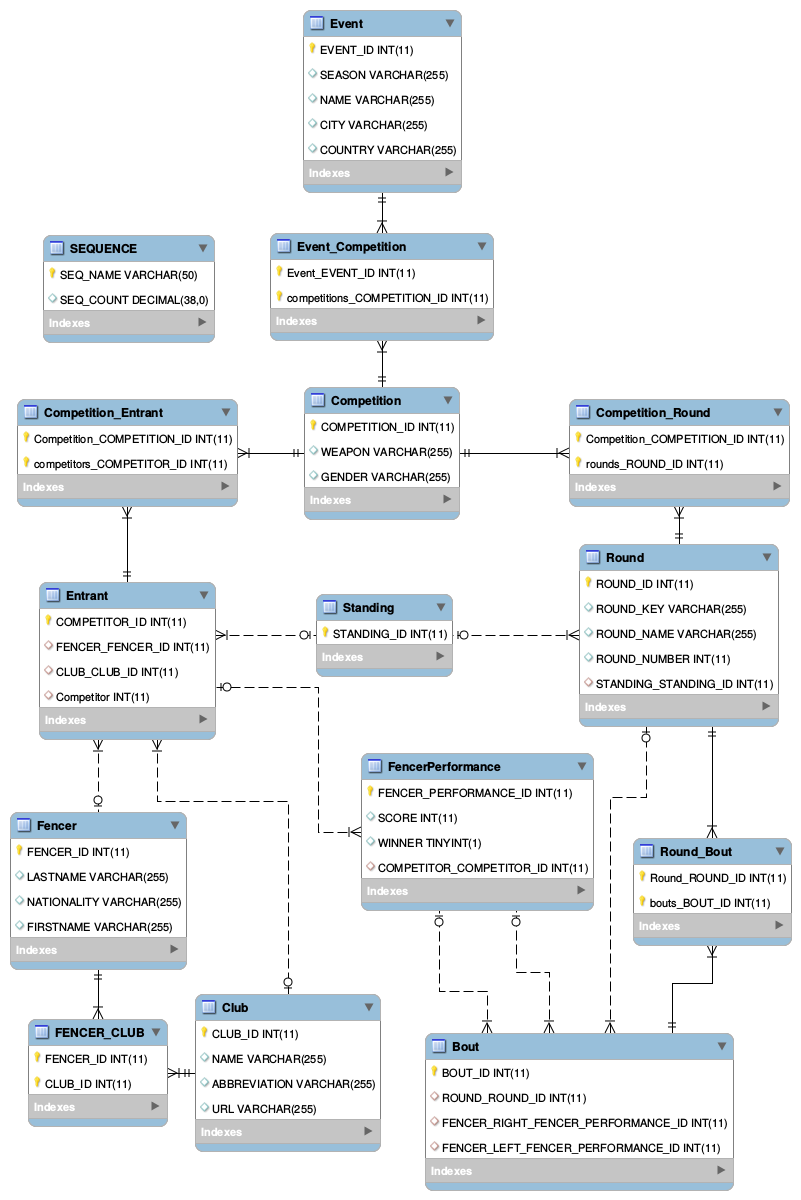
\includegraphics[width=15cm]{db-model.png}
  \caption{Database ER Model - as generated by MySQL Workbench}
  \label{fig:databaseERDesignGenerated}
\end{figure}

\chapter{Work Done}

\section{<Section title>}

\subsection{<Sub-section title>}

\subsection{<Sub-section title>}
some text\citep{einstein}, some more text
\subsection{<Sub-section title>}

\subsection{<Sub-section title>}

Refer figure \ref{fig:label}.

\begin{figure}[htb]
\centering

\includegraphics[scale=0.3]{glider} % e.g. insert ./image for image.png in the working directory, adjust scale as necessary
\caption{<Caption here>}
\label{fig:label} % insert suitable label, this is used to refer to a fig from within the text as shown above
\end{figure}

\subsection{<Sub-section title>}


\section{<Section title>}


\section{Source Code}

\definecolor{mygreen}{rgb}{0,0.6,0}
\definecolor{mygray}{rgb}{0.5,0.5,0.5}
\definecolor{annotationgray}{rgb}{0.25,0.25,0.25}
\definecolor{mymauve}{rgb}{0.58,0,0.82}

\lstset{ %
  backgroundcolor=\color{white},   % choose the background color; you must add \usepackage{color} or \usepackage{xcolor}
  basicstyle=\footnotesize,        % the size of the fonts that are used for the code
  breakatwhitespace=false,         % sets if automatic breaks should only happen at whitespace
  breaklines=true,                 % sets automatic line breaking
  captionpos=b,                    % sets the caption-position to bottom
  commentstyle=\color{mygreen},    % comment style
  deletekeywords={...},            % if you want to delete keywords from the given language
  escapeinside={\%*}{*)},          % if you want to add LaTeX within your code
  extendedchars=true,              % lets you use non-ASCII characters; for 8-bits encodings only, does not work with UTF-8
  frame=single,	                   % adds a frame around the code
  keepspaces=true,                 % keeps spaces in text, useful for keeping indentation of code (possibly needs columns=flexible)
  keywordstyle=\color{blue},       % keyword style
  language=Java,                 % the language of the code
  morecomment=[s][\color{annotationgray}]{@}{\ },	% for setting @Annotations to
  % grey
  numbers=left,                    % where to put the line-numbers; possible
  % values are (none, left, right)
  numbersep=5pt,                   % how far the line-numbers are from the code
  numberstyle=\tiny\color{mygray}, % the style that is used for the line-numbers
  rulecolor=\color{black},         % if not set, the frame-color may be changed on line-breaks within not-black text (e.g. comments (green here))
  showspaces=false,                % show spaces everywhere adding particular underscores; it overrides 'showstringspaces'
  showstringspaces=false,          % underline spaces within strings only
  showtabs=false,                  % show tabs within strings adding particular underscores
  stepnumber=1,                    % the step between two line-numbers. If it's 1, each line will be numbered
  stringstyle=\color{mymauve},     % string literal style
  tabsize=2,	                   % sets default tabsize to 2 spaces
  title=\lstname                   % show the filename of files included with \lstinputlisting; also try caption instead of title
}

\lstinputlisting{dummy_source.java}

% Trying an XML file
\lstinputlisting[language=XML]{../SportsML-G2/testing/example-2-open.xml}


\cleardoublepage
%\pagebreak
\phantomsection
\addcontentsline{toc}{chapter}{Acknowledgements}
\chapter*{Acknowledgments}
\vspace{1.0in}
<Acknowledgements here>


 

<Name here>

<Month and Year here>
{National Institute of Technology Calicut}
\newpage

\cleardoublepage
%\pagebreak
\phantomsection
\addcontentsline{toc}{chapter}{References}

%\bibliographystyle{agsm}
%\bibliography{references}

%\begin{thebibliography}{99}
%
%\bibitem{citation-1-name-here}<Name of the reference here>,\ \url{<url here>}
%
%\bibitem{citation-2-name-here}<Name of the reference here>,\ \url{<url here>}
%
%\end{thebibliography}


\bibliography{references}

\end{document}
